%
% quadrupol1.tex -- Quadrupolpotential Niveaulinien
%
% (c) 2017 Prof Dr Andreas Müller, Hochschule Rapperswil
%
\documentclass[tikz]{standalone}
\usepackage{times}
\usepackage{txfonts}
\usepackage{fp}
\usepackage{ifthen}
\usepackage[utf8]{inputenc}
\usetikzlibrary{arrows,intersections}
\usetikzlibrary{fixedpointarithmetic}
\begin{document}
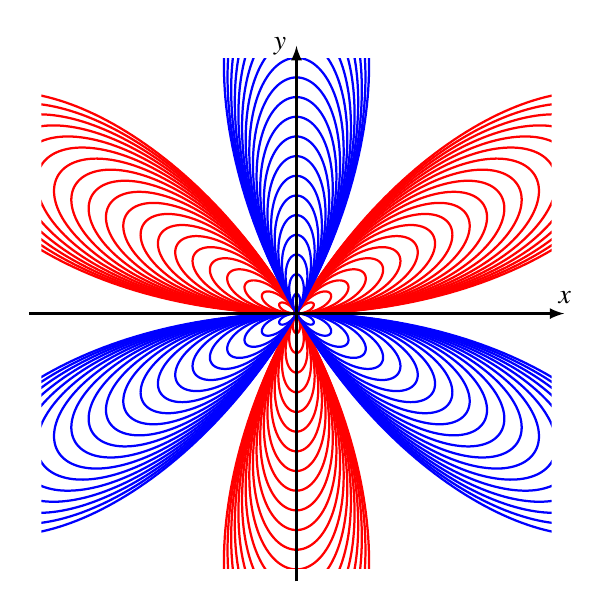
\begin{tikzpicture}[>=latex, thick, scale=2]

\begin{scope}
\clip (-1.62,-1.62) rectangle (1.62,1.62);
\foreach \c in {1,...,20}
{
	\draw[domain=0:360,samples=400,red] plot ({\x}:{\c/2 * sin(3*\x)^1/4});
	\draw[domain=0:360,samples=400,blue] plot ({\x}:{-\c/2 * sin(3*\x)^1/4});
}
\end{scope}

\draw[->] (-1.7,0)--(1.7,0) coordinate[label={above:$x$}];
\draw[->] (0,-1.7)--(0,1.7) coordinate[label={left:$y$}];

\end{tikzpicture}
\end{document}
